% Source: graduate-coursework/Research/Intro_to_Agents/handouts/Part3_Basic_Usage.tex

\documentclass[border=4pt]{standalone}
\usepackage[T1]{fontenc}
\usepackage{graphicx}
\usepackage{lmodern}
\usepackage{tikz}
\usepackage{xcolor}
\usetikzlibrary{shapes.geometric,arrows.meta,positioning,calc,fit,backgrounds,decorations.pathreplacing}

\definecolor{UofSCGarnet}{HTML}{73000a}
\definecolor{UofSCBlack}{HTML}{000000}
\definecolor{UofSCWhite}{HTML}{ffffff}
\definecolor{UofSCRose}{HTML}{CC2E40}
\definecolor{UofSCAtlantic}{HTML}{466A9F}
\definecolor{UofSCCongaree}{HTML}{1F414D}
\definecolor{UofSCHorseshoe}{HTML}{65780B}
\definecolor{UofSCGrass}{HTML}{CED318}
\definecolor{UofSCHoneycomb}{HTML}{A49137}
\definecolor{UofSC90Black}{HTML}{363636}
\definecolor{UofSC70Black}{HTML}{5C5C5C}
\definecolor{UofSC50Black}{HTML}{A2A2A2}
\definecolor{UofSCWarmGrey}{HTML}{676156}
\definecolor{UofSCSandstorm}{HTML}{FFF2E3}
\definecolor{UofSCDarkGarnet}{HTML}{570008}
\definecolor{UofSCAzalea}{HTML}{844247}

\tikzset{
    % Sharp-cornered boxes
    process/.style={
        rectangle,
        draw=UofSCBlack,
        thick,
        fill=UofSCWhite,
        text=UofSCBlack,
        minimum width=3cm,
        minimum height=0.8cm,
        align=center,
        font=\small
    },
    process highlight/.style={
        process,
        fill=UofSCGarnet,
        text=UofSCWhite
    },
    process secondary/.style={
        process,
        fill=UofSCAtlantic,
        text=UofSCWhite
    },
    process tertiary/.style={
        process,
        fill=UofSCCongaree,
        text=UofSCWhite
    },
    arrow/.style={
        ->,
        >=Stealth,
        thick,
        color=UofSCBlack
    },
    arrow garnet/.style={
        arrow,
        color=UofSCGarnet
    },
    label box/.style={
        rectangle,
        draw=none,
        fill=UofSCSandstorm,
        text=UofSCBlack,
        font=\scriptsize,
        align=center
    },
    decision/.style={
        diamond,
        draw=UofSCBlack,
        thick,
        fill=UofSCHoneycomb,
        text=UofSCBlack,
        minimum width=2cm,
        minimum height=1cm,
        align=center,
        font=\small,
        aspect=2
    }
}

\begin{document}
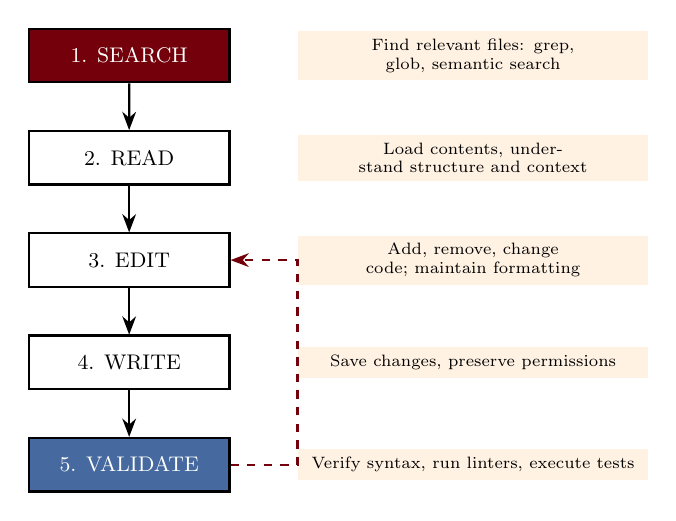
\begin{tikzpicture}[node distance=0.7cm, scale=0.85, transform shape]
        % Vertical flow
        \node[process highlight] (search) {1. SEARCH};
        \node[process, below=of search] (read) {2. READ};
        \node[process, below=of read] (edit) {3. EDIT};
        \node[process, below=of edit] (write) {4. WRITE};
        \node[process secondary, below=of write] (validate) {5. VALIDATE};

        % Descriptions on the right
        \node[label box, right=1cm of search, text width=5cm]
              {Find relevant files: grep, glob, semantic search};
        \node[label box, right=1cm of read, text width=5cm]
              {Load contents, understand structure and context};
        \node[label box, right=1cm of edit, text width=5cm]
              {Add, remove, change code; maintain formatting};
        \node[label box, right=1cm of write, text width=5cm]
              {Save changes, preserve permissions};
        \node[label box, right=1cm of validate, text width=5cm]
              {Verify syntax, run linters, execute tests};

        % Arrows
        \draw[arrow] (search) -- (read);
        \draw[arrow] (read) -- (edit);
        \draw[arrow] (edit) -- (write);
        \draw[arrow] (write) -- (validate);

        % Feedback loop
        \draw[arrow, dashed, color=UofSCGarnet] (validate.east) -- ++(1,0) |- (edit.east);
    \end{tikzpicture}
\end{document}
